\documentclass{ieeeaccess}
\usepackage{cite}
\usepackage{amsmath,amssymb,amsfonts}
\usepackage{algorithmic}
\usepackage{graphicx}
\graphicspath{{Images/}}
\usepackage{textcomp}

\usepackage[english]{babel}
\usepackage[utf8]{inputenc}
\usepackage[T1]{fontenc}
\usepackage{csquotes}
\usepackage{float}
\usepackage{enumerate}
\usepackage{lmodern}

\setlength{\marginparwidth}{2cm}
% \usepackage[disable]{todonotes}
\usepackage[showframe=false]{geometry}
\usepackage{amsthm}
\usepackage{subfiles}

\usepackage{siunitx}
\usepackage{multirow}
\usepackage{lscape}
\usepackage{booktabs}
\usepackage{tabularx} 
\usepackage[nottoc,numbib]{tocbibind}
\usepackage[super]{nth}

\usepackage[colorlinks=true, allcolors=blue]{hyperref}
\usepackage{xurl}

\usepackage{authblk}
\usepackage{changepage}

\usepackage[labelsep=period]{caption}
\usepackage[justification=centering]{caption}
\usepackage{soul}

% \captionsetup[table]{name=TABLE}
\renewcommand{\thetable}{\Roman{table}}

\hyphenation{Block-cha-in}
\hyphenation{block-cha-in}

\setlength\extrarowheight{2pt}

\def\BibTeX{{\rm B\kern-.05em{\sc i\kern-.025em b}\kern-.08em
    T\kern-.1667em\lower.7ex\hbox{E}\kern-.125emX}}

\begin{document}
% \history{Date of publication xxxx 00, 0000, date of current version xxxx 00, 0000.}
\doi{10.1109/ACCESS.2023.0322000}

\title{Non-Fungible Token-based Electronic Voting System - A proposal}
\author{\uppercase{Ricardo Lopes Almeida}\authorrefmark{1,2},
    % \IEEEmembership{Fellow, IEEE},
    Fabrizio Baiardi\authorrefmark{2}, Damiano Di Francesco Maesa\authorrefmark{2}
    \IEEEmembership{Fellow, IEEE},
    % \IEEEmembership{Member, IEEE}
    Laura Ricci\authorrefmark{2} }

\address[1]{Universit\'a di Camerino, 62032 MC, Camerino, Italy (e-mail: ricardo.almeida@unicam.it)}
\address[2]{Dipartimento di Informatica, Universit\'a di Pisa, 56127 PI, Pisa, Italy}

% \tfootnote{This work was supported in part by the U.S. Department of Commerce under Grant BS123456.}

% \markboth
% {Author \headeretal: Preparation of Papers for IEEE TRANSACTIONS and JOURNALS}
% {Author \headeretal: Preparation of Papers for IEEE TRANSACTIONS and JOURNALS}

\corresp{Corresponding author: Ricardo Lopes Almeida (e-mail: ricardo.almeida@unicam.it).}

\begin{abstract}
    % TODO
\end{abstract}

\begin{keywords}
    % TODO
\end{keywords}

\titlepgskip=-21pt

\maketitle

\section{Introduction}
\label{sec:introduction}
\subfile{./Sections/1_Introduction_State_Art.tex}

\section{Background}
\label{background}

% TODO (IF NEEDED)
% \subfile{./Sections/1_Background.tex}
\label{cryptographic_methods}

\twocolumn

\section{Conclusions}
\label{conclusion}
\subfile{./Sections/4_Conclusion.tex}

\bibliographystyle{IEEEtran}
\bibliography{surveyBibliography}

\begin{IEEEbiography}[{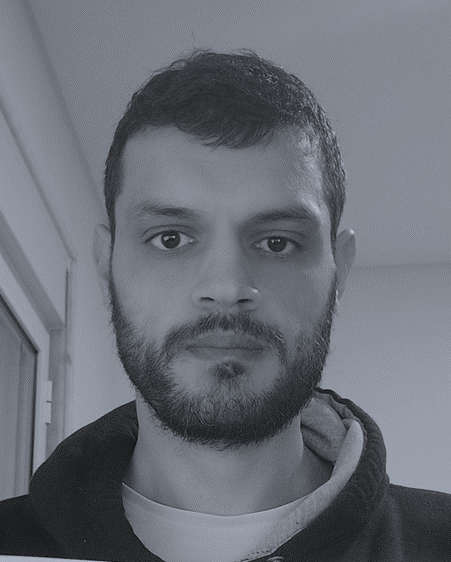
\includegraphics[width=1in,height=1.25in,clip,keepaspectratio]{almei1.png}}]{Ricardo Lopes Almeida} is a doctoral student in the first edition of the Italian Doctoral Programme in Blockchain and Distributed Ledger Technology - Social Systems and Smart Societies at the Univesità di Pisa and Università di Camerino. He obtained an Integrated Master's in Electronic Engineering and Telecommunications from the University of Aveiro, Portugal, in 2012 and a graduation in Physics and Chemistry from the University of \'Evora, Portugal, in 2005.
    \par
    He has split his career almost evenly between academia and industry. He has
    worked as a science teacher in public schools and as a private tutor. After
    acquiring a qualification as an engineer, he has worked mainly as a consulting
    software developer and telecommunications engineer.
\end{IEEEbiography}

\begin{IEEEbiography}[{\includegraphics[width=1in,height=1.25in,clip,keepaspectratio]{baiar1.png}}]{Fabrizio Baiardi} graduated in computer science at Universit\'a di Pisa where he is currently a full professor in computer science.
    \par
    His main research interest is cyber risk assessment and management. He is a
    cofounder of Haruspex, a startup that develops risk assessment and management
    tools based upon adversary emulation. He holds some patents on intrusion
    detection.
\end{IEEEbiography}

\begin{IEEEbiography}[{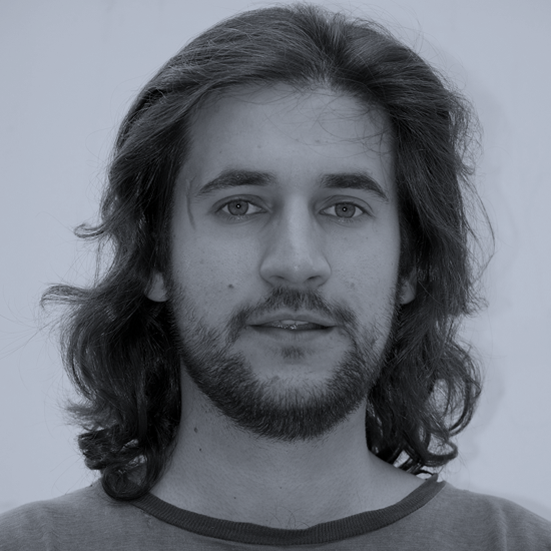
\includegraphics[width=1in,height=1.25in,clip,keepaspectratio]{maesa1.png}}]{Damiano Di Francesco Maesa} is an assistant professor in computer science at the University of Pisa, Italy. His past affiliations include the University of Cambridge, King's College London, and the National Research Institute of Italy.
    \par
    He has a PhD in Computer Science from the University of Pisa and specialises in
    blockchain and Distributed Ledger Technologies (DLT). He has been involved in
    the topic since 2013, and, beside his academic contributions, he has held
    several guest lectures, seminars, and workshops to spread awareness about
    blockchain technology.
\end{IEEEbiography}

\begin{IEEEbiography}[{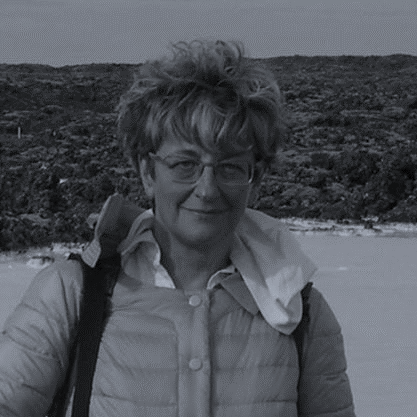
\includegraphics[width=1in,height=1.25in,clip,keepaspectratio]{ricci1.png}}]{Laura Ricci} received the M.Sc. in Computer Science from the University of Pisa in 1983 and the Ph.D. from the same university, in 1990. She is currently a full professor at the Department of Computer Science, University of Pisa, Italy.
    \par
    Her research interests include cryptocurrencies and blockchains, peer-to-peer
    networks, and social network analysis. In these fields, she has co-authored
    150+ papers published in international journals and conference/workshop
    proceedings. She has served as programme committee member and chair of several
    conferences and workshops. She has been involved in several research projects,
    and she is currently the coordinator of the Italian PRIN project "AWESOME:
    Analysis framework for WEb3 SOcial MEdia". She has been a member of the
    National Committee for the definition of the Italian National Strategy for
    Blockchain.
\end{IEEEbiography}

\EOD
\end{document}
